%% 
%% Copyright 2007-2020 Elsevier Ltd
%% 
%% This file is part of the 'Elsarticle Bundle'.
%% ---------------------------------------------
%% 
%% It may be distributed under the conditions of the LaTeX Project Public
%% License, either version 1.2 of this license or (at your option) any
%% later version.  The latest version of this license is in
%%    http://www.latex-project.org/lppl.txt
%% and version 1.2 or later is part of all distributions of LaTeX
%% version 1999/12/01 or later.
%% 
%% The list of all files belonging to the 'Elsarticle Bundle' is
%% given in the file `manifest.txt'.
%% 
%% Template article for Elsevier's document class `elsarticle'
%% with harvard style bibliographic references

\documentclass[3p]{elsarticle}

%% Use the option review to obtain double line spacing
%% \documentclass[authoryear,preprint,review,12pt]{elsarticle}

%% Use the options 1p,twocolumn; 3p; 3p,twocolumn; 5p; or 5p,twocolumn
%% for a journal layout:
%% \documentclass[final,1p,times,authoryear]{elsarticle}
%% \documentclass[final,1p,times,twocolumn,authoryear]{elsarticle}
%% \documentclass[final,3p,times,authoryear]{elsarticle}
%% \documentclass[final,3p,times,twocolumn,authoryear]{elsarticle}
%% \documentclass[final,5p,times,authoryear]{elsarticle}
%% \documentclass[final,5p,times,twocolumn,authoryear]{elsarticle}

%% For including figures, graphicx.sty has been loaded in
%% elsarticle.cls. If you prefer to use the old commands
%% please give \usepackage{epsfig}

%% The amssymb package provides various useful mathematical symbols
\usepackage{amsmath}
\usepackage{caption}
\usepackage{subfig}
\usepackage{float}
\usepackage{booktabs}
\usepackage{tabularx}
\usepackage{tikz}
\usepackage{subfig}
\usepackage{adjustbox}
\usepackage[figuresright]{rotating}
\usepackage{tikz}
\usepackage{multirow}
\usepackage[hidelinks]{hyperref}
\usepackage{makecell}
\usepackage{calc}  % for '\widthof' macro
\usepackage{array} % for 'w' column type
\newlength\myleneiler
\newlength\mylenomega
\usetikzlibrary{shapes,arrows}
\tikzstyle{block} = [rectangle, draw, text width=4.5em, text centered, minimum height=4em]
\tikzstyle{line} = [draw, -latex']
\tikzstyle{decision} = [diamond, draw, text width=4.5em, text centered, inner sep=0pt]
\tikzstyle{cloud} = [draw, ellipse, text width=4.5em, text centered, minimum height=4em]
\usetikzlibrary{shapes, arrows.meta, positioning}
\tikzstyle{startstop} = [rectangle, rounded corners, minimum width=3cm, minimum height=1cm,text centered, draw=black, fill=red!30]
\tikzstyle{io} = [trapezium, trapezium left angle=70, trapezium right angle=110, minimum width=3cm, minimum height=1cm, text centered, draw=black, fill=blue!30]
\tikzstyle{process} = [rectangle, minimum width=3cm, minimum height=1cm, text centered, draw=black, fill=orange!30]
\tikzstyle{decision} = [diamond, minimum width=3cm, minimum height=1cm, text centered, draw=black, fill=green!30]
\tikzstyle{arrow} = [thick,->,>=stealth]
\setlength\myleneiler{(\widthof{Initial Condition (deg)}-4\tabcolsep)/3}
\setlength\mylenomega{(\widthof{Rotational Velocity Commands (rpm)}-4\tabcolsep)/4}


%% The amsthm package provides extended theorem environments
%% \usepackage{amsthm}

%% The lineno packages adds line numbers. Start line numbering with
%% \begin{linenumbers}, end it with \end{linenumbers}. Or switch it on
%% for the whole article with \linenumbers.
%% \usepackage{lineno}

\journal{Franklin Institute}

\begin{document}

\begin{frontmatter}

%% Title, authors and addresses

%% use the tnoteref command within \title for footnotes;
%% use the tnotetext command for theassociated footnote;
%% use the fnref command within \author or \affiliation for footnotes;
%% use the fntext command for theassociated footnote;
%% use the corref command within \author for corresponding author footnotes;
%% use the cortext command for theassociated footnote;
%% use the ead command for the email address,
%% and the form \ead[url] for the home page:
%% \title{Title\tnoteref{label1}}
%% \tnotetext[label1]{}
%% \author{Name\corref{cor1}\fnref{label2}}
%% \ead{email address}
%% \ead[url]{home page}
%% \fntext[label2]{}
%% \cortext[cor1]{}
%% \affiliation{organization={},
%%            addressline={}, 
%%            city={},
%%            postcode={}, 
%%            state={},
%%            country={}}
%% \fntext[label3]{}

\title{Attitude Control of a 3-DoF Quadrotor Platform using a Linear Quadratic Integral Differential Game Approach}

%% use optional labels to link authors explicitly to addresses:
%% \author[label1,label2]{}
%% \affiliation[label1]{organization={},
%%             addressline={},
%%             city={},
%%             postcode={},
%%             state={},
%%             country={}}
%%
%% \affiliation[label2]{organization={},
%%             addressline={},
%%             city={},
%%             postcode={},
%%             state={},
%%             country={}}

\author{Ali BaniAsad}
\ead{ali.baniasad@ae.sharif.edu}
\author{Alireza Sharifi}
\ead{ar.sharifi@sharif.edu}
\author{Reza Pordal}
\ead{R.pordal@yahoo.com}

% \address{Department of Aerospace Engineering
% Sharif University of Technology Tehran, Iran}
% \address{Department of Aerospace Engineering
% Sharif University of Technology Tehran, Iran}
% \address{Department of Aerospace Engineering
% Sharif University of Technology Tehran, Iran}

\author{Hadi Nobahari}
\ead{nobahari@sharif.edu}



\affiliation{organization={Department of Aerospace Engineering Sharif University of Technology},%Department and Organization
            % addressline={}, 
            city={Tehran},
            % postcode={}, 
            % state={},
            country={Iran}}

\begin{abstract}
%% Text of abstract
	In this study, a linear quadratic integral differential game approach is applied to regulate and track the Euler angles for a quadrotor experimental platform using two players. %%%? long and hard to underestand.
	One produces commands for each channel of the quadrotor and
	another generates  the worst disturbance based on the mini-maximization of a quadratic criterion with integral action.
	For this purpose, first, the attitude dynamics of the platform is modeled and its parameters are identified based on the Nonlinear Least Squares Trust-Region Reflective method.
	The performance of the proposed controller is evaluated for regulation and tracking problems.
	The ability of the controller is also examined in the disturbance rejection.
	Moreover, the influence of uncertainty modeling is studied on the obtained results.
	Then, performance of the proposed controller is compared with the classic Proportional Integral Derivative, Linear Quadratic Regulator, and Linear Quadratic Integral Regulator. The results demonstrate the effectiveness of the Game Theory on the Linear Quadratic Regulator approach when the input disturbance occurs.
\end{abstract}

%%Graphical abstract
\begin{graphicalabstract}
%\includegraphics{grabs}
\end{graphicalabstract}

%%Research highlights
% \begin{highlights}
% \item Research highlight 1
% \item Research highlight 2
% \end{highlights}

\begin{keyword}
%% keywords here, in the form: keyword \sep keyword

%% PACS codes here, in the form: \PACS code \sep code
Linear Quadratic controller \sep Differential Game Theory \sep Quadrotor  \sep 3-DoF Experimental Platform \sep Attitude Control. %%%? check --
%% MSC codes here, in the form: \MSC code \sep code
%% or \MSC[2008] code \sep code (2000 is the default)

\end{keyword}

\end{frontmatter}

%% \linenumbers

%% main text
\section{Introduction}\label{sec:intro}
% In this paper, an LQIR method, called LQIR-DG controller is suggested to produce the optimal and robust control command, i.e. rotational velocity command using the game theory approach.
% Since the LQIR-DG controller is affected by an exact model of the plant, the quadrotor's experimental platform is modeled and its parameters are identified based on experimental data. 
% For control purposes, its linear state-space form is extracted using linearization of the nonlinear UAV.
% then, the LQIR-DG technique is applied in real-time to the experimental platform.
% The performance of the LQIR-DG method is evaluated in the presence of the disturbance and modeling error for regulation and tracking purposes.
% A comparison is also performed between the results of classical PID, LQR, and LQIR and the proposed approach in real-time mode.
% The results show the proposed control structure is effective in the control of the quadrotor platform.
\noindent Quadrotors are a type of Vertical Unmanned Aerial Vehicle (VUAV), that have various applications such as investigation, strategic operation, optical sensing, and entertainment.
The safe flight of the quadrotor in the presence of disturbances relies on a precise control. 
A crucial subsystem of a control system for the quadrotor is the Attitude Control System (ACS). 
To regulate the quadrotor attitude, a Proportional Integral Derivative (PID) controller is utilized in \cite{article_Abdul, article_Bolandi}. Due to the nonlinearity dynamics of the quadrotor, the PID strategy is not effective in the presence of the disturbance and modeling error.
To provide a faster control command in facing the modeling error and reduce the disturbance effect in the attitude control, the model-based control strategies including nonlinear control, intelligent control, optimal control, and robust control have been implemented on the ACS of the quadrotor.

Synergetic Control \cite{article_Chara}, Feedback Linearization (FBL) \cite{article_Aboudonia}, and Sliding Mode Control (SMC) \cite{7007285}, which are a group of the nonlinear control category, have been utilized to regulate the Euler angles (roll, pitch, and yaw angles) of the quadrotor. To control attitude of the quadrotor intelligently, the controller strategies such as reinforcement learning \cite{LIN2020135}, iterative learning \cite{electronics10202474}, machine learning \cite{4564736}, and fuzzy logic \cite{KIM20211888} have been implemented. Moreover, to produce the optimal control commands, the controller strategies including Linear Quadratic Gaussian (LQG) \cite{7367782}, Linear Quadratic Regulator (LQR) \cite{7064553_LQR}, Linear Quadratic Integra Regulator (LQIR) \cite{article_LQIR}, and Model Predictive Controller (MPC) approaches \cite{XUE20227992} have been implemented on a quadrotor.

In the robust control strategies, $H_{\infty}$, $\mu\text{-synthesis}$, and Linear Quadratic Regulator Differential Game (LQR-DG) \cite{10025263} have also been utilized to stabilize the Euler angles of the quadrotor using the mini-maximization of a quadratic criterion including control effort and regulation performance in a worst-case scenario. In the LQR-DG controller \cite{GLIZER201522, 6160768}, the control signals are produced using a pursuit-evasion game, one player tracks the best command, and second player generates the input disturbance. For eliminating the steady-state error, the LQR-DG controller with integral action, called LQIR-DG, is implemented on a model of the ship \cite{6957349}.

In this paper, an LQIR-DG method is implemented real-time on 3-DoF experimental platform of the quadrotor to produce the robust control commands, i.e. rotational velocity of the quadrotor.
To this end, first, the experimental platform of the quadrotor is modeled using the Newton-Euler formulation and its linear state-space form is derived.
Then, the parameters of the quadrotor are estimated by matching experimental data with results from the model simulation.
In the next step, the proposed controller is implemented on the Arduino Mega2560 board using the embedded coder platform in the MATLAB and its performance is investigated in regulation and tracking problems.
Moreover, the rejection capability of the input disturbance and modeling error is tested.
Finally, a comparison is also performed between the results of classical PID, LQR, and LQIR with the proposed method. The results demonstrate that this method has an excellent performance in the attitude control of the quadrotor platform.
A demo video of the results is available online
\href{https://drive.google.com/drive/folders/1DIJs3wmIpmwI8slyHeitA6Ebe-khKTCt?usp=share_link}{here}.


This research is organized as follows: the problem statement is presented in section \ref{sec:problem}. In section \ref{sec:modeling}, the dynamic
platform is modeled. Then, the presented controller architecture is denoted in section \ref{sec:controller}. The numerical results and a conclusion are represented in sections \ref{sec:results} and
\ref{sec:conclusion}, respectively.


% This research is organized as follows: section \ref{sec:problem} presents the problem statement.
% In section \ref{sec:modeling}, the dynamic platform is modeled. Then, the presented controller architecture is denoted in section \ref{sec:controller}. 
% In sections \ref{sec:results} and \ref{sec:conclusion}, numerical results and a conclusion are represented, respectively.

\section{Problem Statement}\label{sec:problem}
\noindent The experimental quadrotor platform rotates freely with rotational velocity ($\Omega_i, i = 1, 2, 3, 4$) about its roll, pitch, and yaw axes, according to Figure \ref{fig:quadrotor}.
The angular velocities in the body frame $(p, q, r)$ and the Euler angles $(\phi, \theta, \psi)$ are measured using an Attitude Heading Reference System (AHRS).
The measured states are utilized in the structure of the proposed controller to stabilize the quadrotor platform.
The graphical abstract of the LQIR-DG controller strategy is depicted in Figure \ref{fig:blockdiagram}.
\begin{figure}[H]
    \centering
    \includegraphics[width=0.7\textwidth]{../Figure/3DOFQuad.png}
    \caption{3-DoF Quadrotor platform.}
    \label{fig:quadrotor}
 \end{figure}
 
 \begin{figure}[H]
    \centering
    \includegraphics[width=0.7\textwidth]{../Figure/schematic.pdf}
    \caption{Graphical abstract of the LQIR-DG controller.}
    \label{fig:blockdiagram}
 \end{figure}
 \section{Model of the Quadrotor Platform}\label{sec:modeling}
 \noindent Here, the quadrotor platform is modeled as nonlinear.
 Then, a state-space model and a linear model are developed for control purposes to be utilized in the controller strategy.
 Finally, a nonlinear identification method is applied to identify the parameters of the quadrotor.
 \subsection{Quadrotor Configuration}
 \noindent According to Figure \ref{fig:schematic}, the 3-DoF quadrotor schematic is including four rotors rotating the $z_B$ axis in the body frame with a rotational velocity, $\Omega_i~(i=1, 2, 3, 4)$. To eliminate the yawing moment, rotors (2, 4) and (1, 3) rotate clockwise and counter counterclockwise, respectively.

% \noindent Figure \ref{fig:schematic} shows the quadrotor schematic. It depicts four rotors rotating around the $z_B$ axis in the coordinate system of the body. The rotors have a rotational velocity of $\Omega_r$.
% The quadrotor platform has 3 degrees of freedom, including roll, pitch, and yaw motions, which are described by roll $(\phi)$, pitch $(\theta)$, and yaw $(\psi)$ angles, respectively. %%%? two roll, pitch, yaw
% To counteract the yawing moment, rotors 1 and 3 rotate counterclockwise, while rotors 2 and 4 rotate clockwise. This configuration is designed to cancel out the torque generated by the propellers and stabilize the quadrotor platform. %%%? write by my self and hace many similarity
\begin{figure}[H]
    \centering
    \includegraphics[width=12cm]{../Figure/schematic.png}
    \caption{Quadrotor Configuration.}
    \label{fig:schematic}
\end{figure}
\subsection{Dynamic Modeling of the Quadrotor Platform}
\noindent Here, according to Newton-Euler, the model of the quadrotor platform is presented as follows \cite{4399042, article_Bouabdallah}:
\begin{align}
&\dot p = \dfrac{\mathrm{I}_{\text{yy}} - \mathrm{I}_{\text{zz}}}
{\mathrm{I}_{\text{xx}}} qr + q \dfrac{\mathrm{I}_{\text{rotor}}}
{\mathrm{I}_{\text{xx}}}\Omega_{c, r} + \dfrac{\mathrm{b\,d}_{\text{cg}} (\Omega_{c, 2}^2 - \Omega_{c, 4}^2)}{\mathrm{I}
_{\text{xx}}} + \dfrac{d_{\text{roll}}}{\mathrm{I}_{\text{xx}}}
\\
&\dot q = \dfrac{\mathrm{I}_{\text{zz}} - 
\mathrm{I}_{\text{xx}}}{\mathrm{I}_{\text{yy}}} rp +
p \dfrac{\mathrm{I}_{\text{rotor}}}{\mathrm{I}_{\text{xx}}}\Omega_{c, r} + 
\dfrac{\mathrm{b\,d}_{\text{cg}} (\Omega_{c, 1}^2 - \Omega_{c, 3}^2)}{\mathrm{I}_{\text{yy}}} +
\dfrac{d_{\text{pitch}}}{\mathrm{I}_{\text{yy}}}
\\
&\dot r = \dfrac{\mathrm{I}_{\text{xx}} -
\mathrm{I}_{\text{yy}}}{\mathrm{I}_{\text{zz}}} pq 
+  \dfrac{\mathrm{d} (\Omega_{c, 1}^2 - \Omega_{c, 2}^2 + \Omega_{c, 3}^2 - \Omega_{c, 4}^2)}{\mathrm{I}_{\text{zz}}} 
+ \dfrac{d_{\text{yaw}}}{\mathrm{I}_{\text{zz}}}
\end{align}
where $\Omega_{c, i}~(i=1, 2, 3, 4)$ is the rotational velocity, computed as
\begin{align}
    \Omega_{c, 1}^2 &= \Omega_{\text{mean}}^2 + \dfrac{1}{2\mathrm{b\,d}_{\text{cg}}}u_{\text{pitch}} + \dfrac{1}{4d}u_{\text{yaw}} \\
    \Omega_{c, 2}^2 &= \Omega_{\text{mean}}^2 + \dfrac{1}{2\mathrm{b\,d}_{\text{cg}}}u_{\text{roll}} - \dfrac{1}{4d}u_{\text{yaw}}\\
    \Omega_{c, 3}^2 &= \Omega_{\text{mean}}^2 - \dfrac{1}{2\mathrm{b\,d}_{\text{cg}}}u_{\text{pitch}} + \dfrac{1}{4d}u_{\text{yaw}} \\
    \Omega_{c, 4}^2 &= \Omega_{\text{mean}}^2 - \dfrac{1}{2\mathrm{b\,d}_{\text{cg}}}u_{\text{roll}} - \dfrac{1}{4d}u_{\text{yaw}}
\end{align}
In the above equation, $\Omega_{\text{mean}}$ is the rotational velocity of the rotors. Also, $\mathrm{d}_{\text{cg}}$, $\text{d}$, and $\text{b}$ represent the distance between the rotors and the gravity center, drag factor, and thrust factor, respectively.
$d_{\text{roll}}$, $d_{\text{pitch}}$, and $d_{\text{yaw}}$ denote the disturbances produced in the body coordinate frame. Additionally,
$u_{\text{roll}}$, $u_{\text{pitch}}$, and $u_{\text{yaw}}$ are control commands generated by the LQIR-DG controller. $\mathrm{I}_{\text{rotor}}$ is rotor inertia, and $\mathrm{I}_{\text{xx}}$, $\mathrm{I}_{\text{yy}}$, and $\mathrm{I}_{\text{zz}}$ are the moments of inertia.
Euler angle rates are also determined from angular body rates as follows:
\begin{equation}
	\begin{bmatrix}
	\dot\phi \\
	\dot\theta \\
	\dot\psi
	\end{bmatrix} = 
	\begin{bmatrix}
	1 & \sin(\phi)\tan(\theta) & \cos(\phi)\tan(\theta) \\
	0 & \cos(\phi) & -\sin(\phi) \\
	0 & \sin(\phi)/\cos(\theta) & \cos(\phi)/\cos(\theta)
	\end{bmatrix}
	\begin{bmatrix}
	p \\
	q \\
	r
	\end{bmatrix}
\end{equation}
The residual rotor velocity, denoted by $\Omega_{c,r}$, is calculated as follows:
\begin{equation}
	\Omega_{c, r} = -\Omega_{c, 1} + \Omega_{c, 2} - \Omega_{c, 3} + \Omega_{c, 4}
\end{equation}

\subsection{State-Space Formulation}\label{sec:state-space}
\noindent By defining $\boldsymbol{\mathrm{x}}_{\text{roll}} = \begin{bmatrix}
	x_1 & x_2
\end{bmatrix}^{\mathrm{T}}=
\begin{bmatrix}
	p & \phi
\end{bmatrix}^{\mathrm{T}}$
,
$\boldsymbol{\mathrm{x}}_{\text{pitch}} = \begin{bmatrix}
	x_3 & x_4 \end{bmatrix}^{\mathrm{T}} = 
	\begin{bmatrix}
	q & \theta \end{bmatrix}^{\mathrm{T}}
	$
	, and 
	$\boldsymbol{\mathrm{x}}_{\text{yaw}} = 
	\begin{bmatrix}
		x_5 & x_6
	\end{bmatrix}^{\mathrm{T}} = 
	\begin{bmatrix}
		r & \psi
	\end{bmatrix}^{\mathrm{T}}$, the formulation of the quadrotor platform is presented as follows:
\begin{align}\label{eq:diffeq}
	\dot x_1 &= \Gamma_1x_3 x_5 + \Gamma_2 x_3 \Omega_r + \Gamma_3\mathrm{b\,d}_{\text{cg}} (\Omega_{c, 1}^2 - \Omega_{c, 3}^2) + \Gamma_3d_{\text{roll}} \\[0.5em]
	\dot x_2 &= x_1 + (x_3\sin(x_2) + x_3\cos(x_2))\tan(x_4)
    \\[0.5em]
    \dot x_3 &= \Gamma_4 x_1 x_5 - \Gamma_5 x_1 \Omega_r +  \Gamma_6\mathrm{b\,d}_{\text{cg}} (\Omega_{c, 2}^2 - \Omega_{c, 4}^2) + \Gamma_6d_{\text{pitch}}\\[0.5em] \label{eq:diffeq-mid}
	\dot x_4 &= x_3\cos(x_4) - x_5\sin(x_2)\\[0.5em]
    \dot x_5 &= \Gamma_7x_1 x_3 +  \Gamma_8\mathrm{d} (\Omega_{c, 1}^2 - \Omega_{c, 2}^2 + \Omega_{c, 3}^2 - \Omega_{c, 4}^2) + \Gamma_8d_{\text{yaw}}\\[0.5em] 
    \dot x_6 &= (x_3\sin(x_4) + x_5\cos(x_2))/\cos(x_4) \label{eq:diffeq-end}
\end{align}
where $\Gamma_i (i = 1, \ldots, 8)$ is defined as
\begin{equation}
	\begin{split}
		\Gamma_1 &= \dfrac{\mathrm{I}_{\text{yy}} - \mathrm{I}_{\text{zz}}}{\mathrm{I}_{\text{xx}}}, \quad \Gamma_2 = \dfrac{\mathrm{I}_{\text{rotor}}}{\mathrm{I}_{\text{xx}}}, \quad \Gamma_3 = \dfrac{1}{\mathrm{I}_{\text{xx}}}\\ \Gamma_4 &= \dfrac{\mathrm{I}_{\text{zz}} - \mathrm{I}_{\text{xx}}}{\mathrm{I}_{\text{yy}}}, \quad \Gamma_5 = \dfrac{\mathrm{I}_{\text{rotor}}}{\mathrm{I}_{\text{xx}}}, \quad \Gamma_6 = \dfrac{1}{\mathrm{I}_{\text{yy}}} \\ \Gamma_7 &= \dfrac{\mathrm{I}_{\text{xx}} - \mathrm{I}_{\text{yy}}}{\mathrm{I}_{\text{zz}}}, \quad \Gamma_8 = \dfrac{1}{\mathrm{I}_{\text{zz}}}
	\end{split}
\end{equation}
The measurement vector, obtained from the AHRS, is presented as follows:
\begin{equation}
    \begin{split}
        \boldsymbol{\mathrm{z}} &= \begin{bmatrix}
        p \
        q \
        r \
        \phi \
        \theta \
        \psi
    \end{bmatrix}^\mathrm{T} + \boldsymbol{\nu}
    \end{split}
\end{equation}
where $\boldsymbol{\nu}$ is a Gaussian white noise. Moreover, the superscripts $\mathrm{T}$ indicate the transpose notation.
%%%? capital or small G g ? 
\subsection{Linear Model}
\noindent By defining $\boldsymbol{\dot{\mathrm{x}}} = \begin{bmatrix}
	\boldsymbol{{\mathrm{\dot x_{\text{roll}}}}}&
	\boldsymbol{{\mathrm{\dot x_{\text{pitch}}}}}&
	\boldsymbol{{\mathrm{\dot x_{\text{yaw}}}}}
\end{bmatrix}^{\mathrm{T}}$, the linear model of the quadrotor platform represented about the equilibrium points $(\boldsymbol{{\mathrm{x}}}_e^*\!=\!0$ and $\boldsymbol{{\mathrm{u}}}_e^*\!=\!0)$ as
\begin{equation}\label{eq:linear}
	\boldsymbol{\dot{\mathrm{x}}} = \boldsymbol{\mathrm{A\,x}} + 
	\boldsymbol{\mathrm{B}}
	\left(\boldsymbol{\mathrm{u}} + \boldsymbol{\mathrm{d}}\right)
\end{equation}
$\boldsymbol{\mathrm{A}}$ is the dynamic system matrix, denoted as
\begin{equation}
	\boldsymbol{\mathrm{A}} = \begin{bmatrix}
		\boldsymbol{{\mathrm{A_{\text{roll}}}}} & \boldsymbol{0} & \boldsymbol{0}\\
		\boldsymbol{0} & \boldsymbol{{\mathrm{A_{\text{pitch}}}}} & \boldsymbol{0} \\
		\boldsymbol{0} & \boldsymbol{0} & \boldsymbol{{\mathrm{A_{\text{yaw}}}}}
	\end{bmatrix}
\end{equation}
$
		\boldsymbol{\mathrm{A}}_{\text{roll}}  =\boldsymbol{\mathrm{A}}_{\text{pitch}}  = \boldsymbol{\mathrm{A}}_{\text{yaw}}  = \begin{bmatrix}
			0 & 0\\
			1 & 0
		\end{bmatrix}
$. Also, $\boldsymbol{\mathrm{B}}$ is the input matrix defined as
\begin{equation}
	\boldsymbol{\mathrm{B}} =
	\begin{bmatrix}
		\boldsymbol{{\mathrm{B_{\text{roll}}}}} & \boldsymbol{0} & \boldsymbol{0}\\
		\boldsymbol{0} & \boldsymbol{{\mathrm{B_{\text{pitch}}}}} & \boldsymbol{0} \\
		\boldsymbol{0} & \boldsymbol{0} & \boldsymbol{{\mathrm{B_{\text{yaw}}}}}
	\end{bmatrix}
\end{equation}
where $\boldsymbol{\mathrm{B}}_{\text{roll}}  = \begin{bmatrix}
	\dfrac{1}{\mathrm{I}_{\text{xx}}}
	&
	0
\end{bmatrix}^{\mathrm{T}}$, $\boldsymbol{\mathrm{B}}_{\text{pitch}}  = \begin{bmatrix}
	\dfrac{1}{\mathrm{I}_{\text{yy}}}
	&
	0
\end{bmatrix}^{\mathrm{T}}$, and $\boldsymbol{\mathrm{B}}_{\text{yaw}}  = \begin{bmatrix}
	\dfrac{1}{\mathrm{I}_{\text{zz}}}
	&
	0
\end{bmatrix}^{\mathrm{T}}$.
\subsection{Identification of the Platform Parameters}
\noindent In this section, the Nonlinear Least Squares (NLS) algorithm is utilized for estimating the model parameters ($\boldsymbol{\mathrm{\Gamma}}$) of the 3-DoF experimental platform using experimental data.
This technique is based on the Trust-Region Reflective (TRR) method, which finds the best values for $\boldsymbol{\mathrm{\Gamma}}$ by minimizing a cost function, defined as
\begin{equation}
	\min_{\Gamma}\left(\parallel e(\Gamma) \parallel^2\right) = 
	\min_{\Gamma} \left(\sum_{j=1}^{n}(\boldsymbol{z}_j- \tilde{\boldsymbol{z}}_j)(\boldsymbol{z}_j- \tilde{\boldsymbol{z}}_j)^\mathrm{T}\right)
\end{equation} %%%? what is j ??
where $\boldsymbol{z}$ and $\tilde{\boldsymbol{z}}$ are the experimental and simulated output signals when the same input signals are applied.
Moreover, $n$ is the number of scenarios.
To find a vector $\Gamma$, the optimization process performs until convergence is achieved. %%%?
The structure of the identification approach is illustrated in figure \ref{fig:identification}.

\begin{figure}[H]
	\centering
    \resizebox{1\textwidth}{!}{
	\begin{tikzpicture}[font=\small,thick]
		% Start block
		\node[draw, align=center,		minimum width=2.5cm,		minimum height=1cm, fill=blue!10] (block1) {\textbf{Experimental Data} \\Input: rotational velocity\\
		Output: attitude};
			
		% Voltage and Current Measurement
		\node[draw, align=center,		below=of block1,		minimum width=3.5cm,		minimum height=1cm, fill=blue!10	] (block2) {\textbf{Data Preprocessing} \\ Synchronization experimental, vs simulated data.};
		
		% Power and voltage variation
		
		\node[draw, align=center,		below=of block2,		minimum width=3.5cm,		minimum height=1cm, fill=blue!10	] (block3) {\textbf{NLS-TRR Optimization}\\
		Set bounds for parameters\\
		The set initial seed for all parameters\\
		Minimization of the cost function.};

		\node[draw, align=center,	below right=of block3,	minimum width=3cm,	minimum height=2.5cm,	fill=green!10	] (block_p) {{Identified parameters}\\
		$\boldsymbol\Gamma = \begin{bmatrix}\Gamma_1 &
			\Gamma_2 & \Gamma_3 & \Gamma_4\\
			\Gamma_5 & \Gamma_6 & \Gamma_7 & \Gamma_8
		\end{bmatrix}$};

		\node[draw, align=center,	below left=of block3,	minimum width=3cm,	minimum height=2.5cm,	fill=red!10	] (block_s) {{simulated model}\\\includegraphics[scale=.05]{../Figure/All-six.png}};
		
		% Conditions test
		\node[draw,		diamond,		below =4cm of block3,		minimum width=2.5cm,		inner sep=0,		fill=yellow!10	] (block4) { Error $< \delta$};
		
		\node[draw,		below=1.5cm of block4,		minimum height=1cm,		minimum width=2.5cm,		inner sep=0,		fill=blue!10	] (block5) {End};
		
		\node[draw,		right=2cm of block4,		minimum height=1cm,		minimum width=2.5cm,		fill=red!10		] (block6) {Insufficient experimental data};
				
		 
		 
		% Arrows
		\draw[-latex] (block1) edge (block2)
			(block2) edge (block3)
			(block3) -| (block_s);
			% (block3) edge (block_p);
	
		\draw[-latex] (block3) -| (block_p);
	
		\draw[-latex] (block_s) -| (block4);
	
		\draw[-latex] (block_p) -| (block4);
	
		\draw[stealth-stealth] (block_s) -- (block_p);
		 
		\draw[-latex] (block4) -- (block5)
			node[pos=0.5,fill=white,inner sep=0]{Yes};
		 
		\draw[-latex] (block4) -- (block6)
			node[pos=0.5,fill=white,inner sep=0]{No};
	
		\coordinate[left=5.5cm of block3] (aux);
		\coordinate[right= of block_p] (aux1);
		% \draw[-latex] (block6) |- (block2);
		\draw[-latex] (block1) -| (aux) |- (block4);
		\draw[-latex] (block6) -| (aux1) |- (block1);
		\end{tikzpicture}
        }
		\caption{Structure of TRRLS identification approach.}
		\label{fig:identification}
\end{figure}
\section{LQIR-DG Controller Structure}\label{sec:controller}
\noindent First, the augmented states of the quadrotor platform, including the states and their integrals are selected to use in the structure of the LQIR-DG controller for eliminating the steady states errors. Then, the design methodology of the controller structure is introduced to produce the best commands for the 3-DoF quadrotor platform.
\subsection{Augmented States}
\noindent To augment an integral action into the control strategy architecture, the augmented states are defined as $\boldsymbol{\mathrm{x_{a}}} = \begin{bmatrix}
	\boldsymbol{\mathrm{x}} &
	\displaystyle\int\boldsymbol{\mathrm{x}}
\end{bmatrix}^\mathrm{T}$. Then, the quadrotor platform model, utilized in the controller structure, is presented as

\begin{equation}\label{systemlqidg}
	\begin{split}
		\boldsymbol{\dot{\mathrm{x}}_a} &= \begin{bmatrix}
			\boldsymbol{\mathrm{A}} & \boldsymbol{0}\\
			\boldsymbol{\mathrm{I}} & \boldsymbol{0}
		\end{bmatrix}\boldsymbol{\mathrm{x_a}} + \begin{bmatrix}
			\boldsymbol{\mathrm{B}}\\
			\boldsymbol{0}
		\end{bmatrix}
		 \left(\boldsymbol{\mathrm{u}} + \boldsymbol{\mathrm{d}}\right)%, \quad \boldsymbol{x}(0) = 
	\end{split}
\end{equation}
The notation $\boldsymbol{\mathrm{I}}$ denotes the identity matrix.
\subsection{LQIR-DG Control Scheme with Integral Action}
\noindent In the proposed controller scheme, two fundamental players are selected in accordance with the game theory approach. The primary player determines the control commands, while another player generates the worst possible disturbance.
To achieve the primary objective, the first player minimizes the following cost function but the other player maximizes it:
\begin{equation}\label{eq:min_max_cost_function}
    \min_{u} \max_{d} J(\boldsymbol{\mathrm{x_{a_i}}}, {d_i}, {u_i})= \min_{d} \max_{u}
     \int_{0}^{\mathrm{t_f}}\biggl (\boldsymbol{\mathrm{x^\mathrm{T}_{a_i}}}  \boldsymbol{\mathrm{Q_i}} \boldsymbol{\mathrm{x_{a_i}}}+
    {{u^\mathrm{T}_i}}  {{R}} {{u_i}}-
    {{d^\mathrm{T}_{i}}} {{ R_{d} d_{i}}}
    \biggl )\mathrm{d}t
\end{equation}
where $\mathrm{t_f}$ is the stop time and $i$-index denotes the roll, pitch, and yaw channels of the quadrotor. $\boldsymbol{\mathrm{Q_i}}$, ${{R_{d}}}$, and ${{R}}$ are weight coefficients of the cost function.
By solving the above problem, the optimal control command is computed as follows \cite{LQDG}:
\begin{equation}
	{{u_i}} = -\boldsymbol{{\mathrm{K}}_{i}} \boldsymbol{{\mathrm{x_{a_i}}}}
\end{equation}
Moreover, the worst disturbance is obtained as
\begin{equation}
	{{d_i}} =\boldsymbol{{\mathrm{K_{d_i}}}}\boldsymbol{{\mathrm{x_{a_i}}}}
\end{equation}
Here, $\boldsymbol{{\mathrm{K_{d_i}}}}$ and $\boldsymbol{{\mathrm{K_i}}}$ are gain values defined as follows:
\begin{align}
	\boldsymbol{{\mathrm{K_{d_i}}}} &= {{{R}}^{-1}_{d}}\boldsymbol{{\mathrm{B}_{a_{d_i}}^\mathrm{T}}}\boldsymbol{{\mathrm{P}}_{a_{d_i}}}\\
	\boldsymbol{{\mathrm{K_i}}} &= {{{R}}^{-1}}\boldsymbol{{\mathrm{B}_{a_i}^\mathrm{T}}}\boldsymbol{{\mathrm{P}}_{a_i}}
\end{align}
$\boldsymbol{{\mathrm{P}}_{a_i}}$ and $\boldsymbol{{\mathrm{P}}_{a_{d_i}}}$ satisfy
\begin{align}\label{coupled_riccatti_LQIDG}
	&-\boldsymbol{\mathrm{A^\mathrm{T}_a}}\boldsymbol{\mathrm{P_{a_{d_i}}}}
	 - \boldsymbol{\mathrm{Q_{i}}} - \boldsymbol{\mathrm{P_{a_{d_i}}}}\boldsymbol{\mathrm{A_a}} 
	 + \boldsymbol{\mathrm{P_{a_{d_i}}}}\boldsymbol{\mathrm{S_{a_i}}}\boldsymbol{\mathrm{P_{a_i}}}
	  +\boldsymbol{\mathrm{P_{a_{d_i}}}}\boldsymbol{\mathrm{S_{a_{d_i}}}}\boldsymbol{\mathrm{P_{a_{d_i}}}}
	=\boldsymbol{\mathrm{0}}\\
            &-\boldsymbol{\mathrm{A^\mathrm{T}_a}}\boldsymbol{\mathrm{P_{a_i}}} - \boldsymbol{\mathrm{Q_i}}
			 - \boldsymbol{\mathrm{P_{a_i}}}\boldsymbol{\mathrm{A_a}}  +
			  \boldsymbol{\mathrm{P_{a_i}}}\boldsymbol{\mathrm{S_{a_{d_i}}}}\boldsymbol{\mathrm{P_{a_{d_i}}}} 
			  +\boldsymbol{\mathrm{P_{a_i}}}\boldsymbol{\mathrm{S_{a_i}}}\boldsymbol{\mathrm{P_{a_i}}} =\boldsymbol{\mathrm{0}}
\end{align}
where $
	\boldsymbol{\mathrm{S_{a_i}}} = \boldsymbol{\mathrm{B_{a_i}}}R^{-1}\boldsymbol{\mathrm{B}^\mathrm{T}_{a_i}}$ and $
	\boldsymbol{\mathrm{S{a_{d_i}}}} = \boldsymbol{\mathrm{B}_{a_{d_i}}}R_{d}^{-1}\boldsymbol{\mathrm{B}^\mathrm{T}_{a_{d_i}}}.
$%%%? needd : or not
\section{Results}\label{sec:results}
\noindent The results of the parameter identification and the LQIR-DG Controller for the quadrotor platform are presented. First, the quadrotor parameters are estimated based on the NLS method. The n,performance of the LQIR-DG structure is evaluated.
Tables \ref{tab:parameters} and \ref{tab:control weight_new} present the quadrotor and LQIR-DG parameters, respectively.
\begin{table}[H]
	\centering
	\caption{Quadrotor parameters}
	\vspace{-0.5cm}
	\renewcommand{\arraystretch}{1.3}
	\begin{center}
	\begin{tabular}{c c c c c c}
	\hline
	Parameter & Unit & Value & Parameter & Unit & Value \\
	\hline
	$\mathrm{d}_{\text{cg}}$ & $\mathrm{m}$ & $0.2$ & $\mathrm{I}_{\text{xx}}$ & $\mathrm{kg.m^2}$ & $0.02839$ \\ 
	$\mathrm{d}$ & $\mathrm{N.m.\sec^2/rad^2}$ & $3.2\times10^{-6}$ &
	$\mathrm{I}_{\text{yy}}$ & $\mathrm{kg.m^2}$ & $0.03066$ \\
	$\mathrm{b}$ & $\mathrm{N.\sec^2/rad^2}$ & $3.13\times10^{-5}$ 
	& $\mathrm{I}_{\text{zz}}$ & $\mathrm{kg.m^2}$ & $0.0439$ \\
	$\Omega_{\text{mean}}$ & $\mathrm{rpm}$ & $2000$ & $\mathrm{I}_{\text{rotor}}$ & $\mathrm{kg.m^2}$ & $4.4398\times 10^{-5}$ \\
	\hline
\end{tabular}
\label{tab:parameters}
\end{center}
\end{table}
\begin{table}[H]
	\centering
	\caption{LQIR-DG controller parameters}
	\renewcommand{\arraystretch}{1.3}
	\begin{tabular}{@{}ccc@{}}
	\toprule
	Channel & Weighting Matrix & Values \\
	\midrule
	Roll & $\mathbf{Q_{roll}}$ & $\text{diag}([0.02, 65.96, 83.04, 0.00])$ \\
	Pitch & $\mathbf{Q_{pitch}}$ & $\text{diag}([435.01, 262.60, 262.60, 0.00])$ \\
	Yaw & $\mathbf{Q_{yaw}}$ & $\text{diag}([4 \times 10^{-4}, 0.00, 0.133, 0])$ \\
	-& $R$ & $1$ \\
	-&$R_d$ & $1.2764$ \\
	\bottomrule
	\end{tabular}
	\label{tab:control weight_new} %%%? R in above is not matrix i have changed
	%%%? need to know where weighting matrix came from
\end{table}
\subsection{Identification of the 3-DoF quadrotor platform model}
\noindent As described in section \ref{sec:state-space}, the parameters of the quadrotor platform, denoted by $\Gamma_i (i=1, ..., 8)$, are identified using the NLS-TRR algorithm.
To increase the accuracy of parameter identification, three scenarios are considered according to Table \ref{tab:identification}.
In the first scenario, depicted in Figure \ref{fig:one_degree_identification}, the quadrotor rotates about only one axis (roll, pitch, or yaw axes) to identify the parameters $\Gamma_3$, $\Gamma_6$, and $\Gamma_8$.
In the second scenario, according to Figure \ref{fig:two_degree_identification}, the parameters $\Gamma_2$ and $\Gamma_5$ are estimated by rotating the experimental platform around its roll and pitch axes simultaneously. Finally, Figure \ref{fig:three_degree_identification} displays the results of the third scenario including the estimation of the parameters $\Gamma_1$, $\Gamma_4$, and $\Gamma_7$ for the UAV model, when the platform freely rotates around three axes.
After the termination condition is met, the optimal values of the quadrotor parameters are computed and denoted in Table \ref{tab:true_parameters}. 
These results illustrate that the outputs of the simulation results for the quadrotor model are consistent with reality.
\begin{table}[H]
	\caption{Scenarios for identification of quadrotor parameters.}
	\centering
	\begin{adjustbox}{max width=\textwidth}
	\begin{tabular}{c c *{3}{wc{\myleneiler}} *{4}{wc{\mylenomega}}}
	\toprule
	\multirow{2}{*}{Scenario} & \multirow{2}{*}{Description}
	& \multicolumn{3}{c}{Initial Condition (deg)} &
	\multicolumn{4}{c}{Rotational Velocity Commands (rpm)} \\
	\cmidrule(lr){3-5} \cmidrule(lr){6-9}
	& & $\phi_0$ & $\theta_0$ & $\psi_0$ & $\Omega_1$ & $\Omega_2$ & $\Omega_3$ & $\Omega_4$\\
	\midrule
	\multirow{3}{*}{I} & roll free & 38 & - & - & 2000 & 2000 & 2000 & 3400\\
	& pitch free & - & -15 & - & 3700 & 2000 & 2000 & 2000 \\
	& yaw free & -& - &-75 & 2000 & 3300 & 2000 & 3300 \\
	\midrule
	II & roll \& pitch free &8 & -5 & - & 1700 & 3800 & 2400 & 1700\\
	\midrule
	III & roll, pitch, \& yaw free &
	8 & -3 & -146 & 1700 & 3800 & 2400 & 1700 \\
	\bottomrule
	\end{tabular}
	\end{adjustbox}
	\label{tab:identification}
\end{table}


\begin{table}[H]
	\renewcommand{\arraystretch}{1.3}
	\caption{True values of the quadrotor parameters.}
	\vspace{-0.5cm}
	\begin{center}
	\begin{tabular}{c c c c}
	\hline
	Parameter & Value & Parameter & Value  \\
	\hline
	$\Gamma_1$ & $-0.9622$ & $\Gamma_5$ & $3.6441\times10^{-4}$ \\

	$\Gamma_2$ & $-0.0154$ & $\Gamma_6$ & $7.5395\times10^{-5}$ \\

	$\Gamma_3$ &$5.4716\times10^{-5}$ & $\Gamma_7$ & $0.1308$ \\

	$\Gamma_4$ & $1.0457$ & $\Gamma_8$ & $4.3753\times10^{-5}$ \\
	\hline
	\end{tabular}
	\label{tab:true_parameters}
	\end{center}
\end{table}
\begin{figure}[H]
	\centering
	\subfloat[]{\includegraphics[width=.45\linewidth]{../Figure/parameter_estimation/roll/roll}\includegraphics[width=.45\linewidth]{../Figure/parameter_estimation/roll/roll_parameter}
	}
	\hfil
	% \vspace{-0.25cm}
	\subfloat[]{\includegraphics[width=.45\linewidth]{../Figure/parameter_estimation/pitch/pitch}\includegraphics[width=.45\linewidth]{../Figure/parameter_estimation/pitch/pitch_parameter}
	}
	\hfil
	% \vspace{-0.25cm}
	\subfloat[]{\includegraphics[width=.45\linewidth]{../Figure/parameter_estimation/yaw/yaw}\includegraphics[width=.45\linewidth]{../Figure/parameter_estimation/yaw/yaw_parameter}
	}
	\caption{Identification process results when the quadrotor rotates about only one axis: (a) Identification of $\Gamma_3$ in free roll motion. (b) Identification of $\Gamma_6$ in free pitch motion. (c) Identification of $\Gamma_8$
	in free yaw motion.}
	\label{fig:one_degree_identification}
\end{figure}
\begin{figure}[H]
	\centering
	\vspace{-2.2cm}
	\subfloat[]{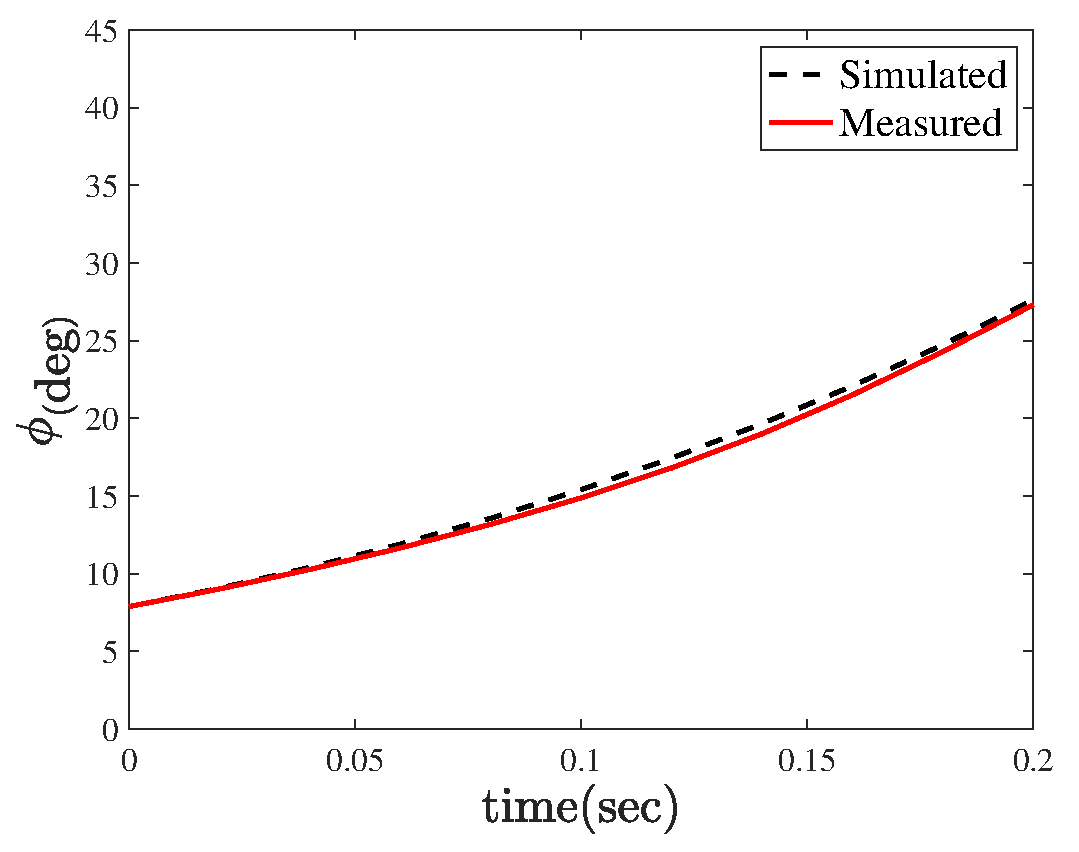
\includegraphics[width=.4\linewidth]{../Figure/parameter_estimation/roll-pitch/roll}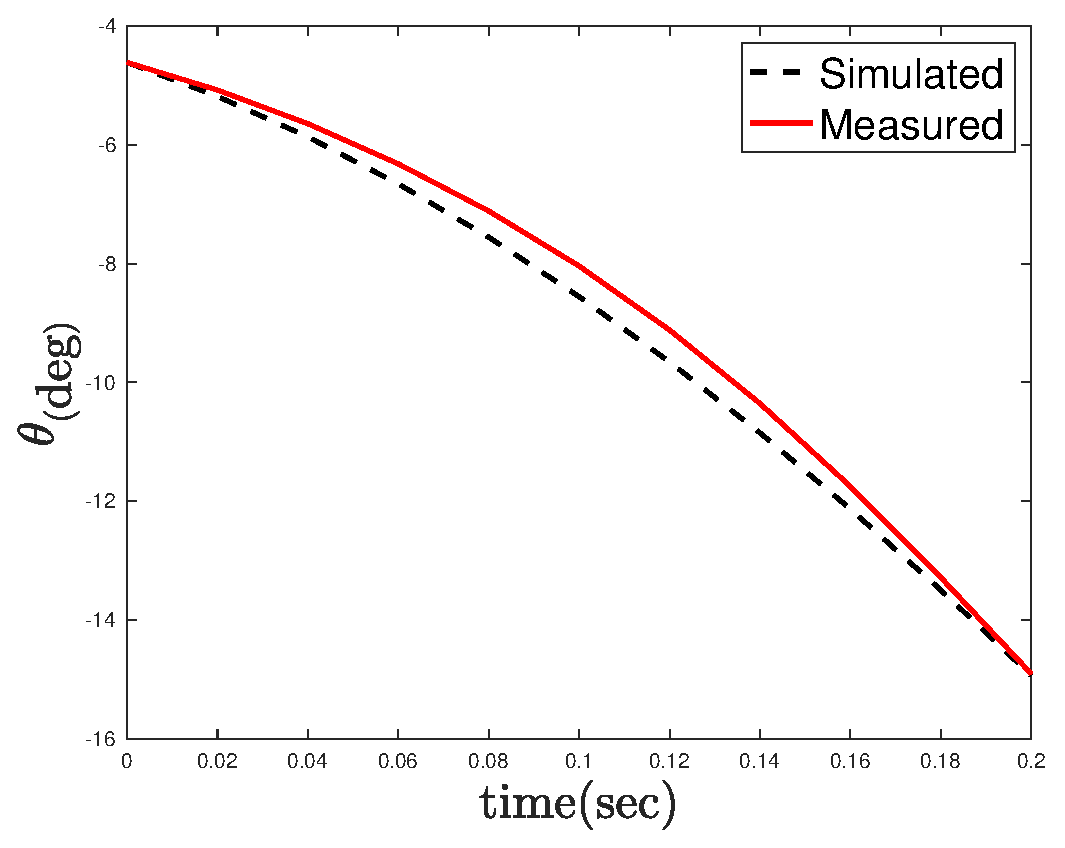
\includegraphics[width=.4\linewidth]{../Figure/parameter_estimation/roll-pitch/pitch}
	}
	\hfil
	% \vspace{-0.25cm}
	\subfloat[]{\includegraphics[width=.4\linewidth]{../Figure/parameter_estimation/roll-pitch/roll_parameter}\includegraphics[width=.4\linewidth]{../Figure/parameter_estimation/roll-pitch/pitch_parameter}
	}
	\caption{Identification process results when the quadrotor rotates about its roll and pitch axes:
	(a) Comparison of Simulation and experimental results. (b) Identification of $\Gamma_2$ and $\Gamma_5$.}
	\label{fig:two_degree_identification}
% \end{figure}
% \begin{figure}[H]
	\centering
	\subfloat[]{\includegraphics[width=.33\linewidth]{../Figure/parameter_estimation/3DOF/roll}\includegraphics[width=.33\linewidth]{../Figure/parameter_estimation/3DOF/pitch}\includegraphics[width=.33\linewidth]{../Figure/parameter_estimation/3DOF/yaw}
	}
	\hfil
	\subfloat[]{\includegraphics[width=.33\linewidth]{../Figure/parameter_estimation/3DOF/roll_parameter}\includegraphics[width=.33\linewidth]{../Figure/parameter_estimation/3DOF/pitch_parameter}\includegraphics[width=.33\linewidth]{../Figure/parameter_estimation/3DOF/yaw_parameter}
	}
	\caption{Identification process results when the quadrotor rotates about its roll, pitch, and yaw axes: (a) Comparison of Simulation and experimental results. (b) Identification of $\Gamma_1$ , $\Gamma_4$ and
	$\Gamma_7$ parameters.}
	\label{fig:three_degree_identification}
\end{figure}
\subsection{Evaluation of LQIR-DG Performance}
\noindent In this section, the LQIR-DG controller algorithm is evaluated in three scenarios i) regulation and tracking problems, ii) disturbance rejection, and iii) impact of model uncertainty.
Finally, a comparison of the proposed controller is performed with a PID controller and variants of the LQR controller. 
The PID controller parameters are presented in Table \ref{tab:PID_parameters}.
\begin{table}[H]
	\renewcommand{\arraystretch}{1.3}
	\caption{PID controller parameters}
	\vspace{-0.5cm}
	\begin{center}
		\begin{tabular}{cccc}
		\hline
		\textbf{Channel} & \textbf{$K_p$} & \textbf{$K_i$} & \textbf{$K_d$} \\
		\hline
		roll & 18 & 6 & 9 \\
		pitch & 22 & 15 & 16 \\
		\hline
		\end{tabular}
		\label{tab:PID_parameters}
	\end{center}
\end{table}
\subsubsection{Investigating of the Regulation and Tracking Problems}\label{sec:regulation}
\noindent The results of the proposed approach are presented for tracking the desired roll and pitch angles in Figures \ref{fig:result} and \ref{fig:omega}.
 %%%? so many of
Figure \ref{fig:result} \ref{sub@fig:regulation} compares the desired and output signals, i.e., the Euler angles during regulation problem. Moreover, Figure \ref{fig:result} \ref{sub@fig:square} compares the desired square wave signals with a frequency of 0.02 Hz and an amplitude of 20 degrees with the output signals, when the quadrotor platform freely rotates around roll and pitch simultaneity.
Figures \ref{fig:omega} \ref{sub@fig:omega_regulation} and \ref{sub@fig:omega_square} show the rotational velocity commands of the quadrotor in the regulation and tracking problems, respectively. These results demonstrate that the roll and pitch angles are accurately controlled by the proposed approach.



\begin{figure}[H]
	\centering
	\vspace{0.3cm}
	\subfloat[\label{fig:regulation}]{{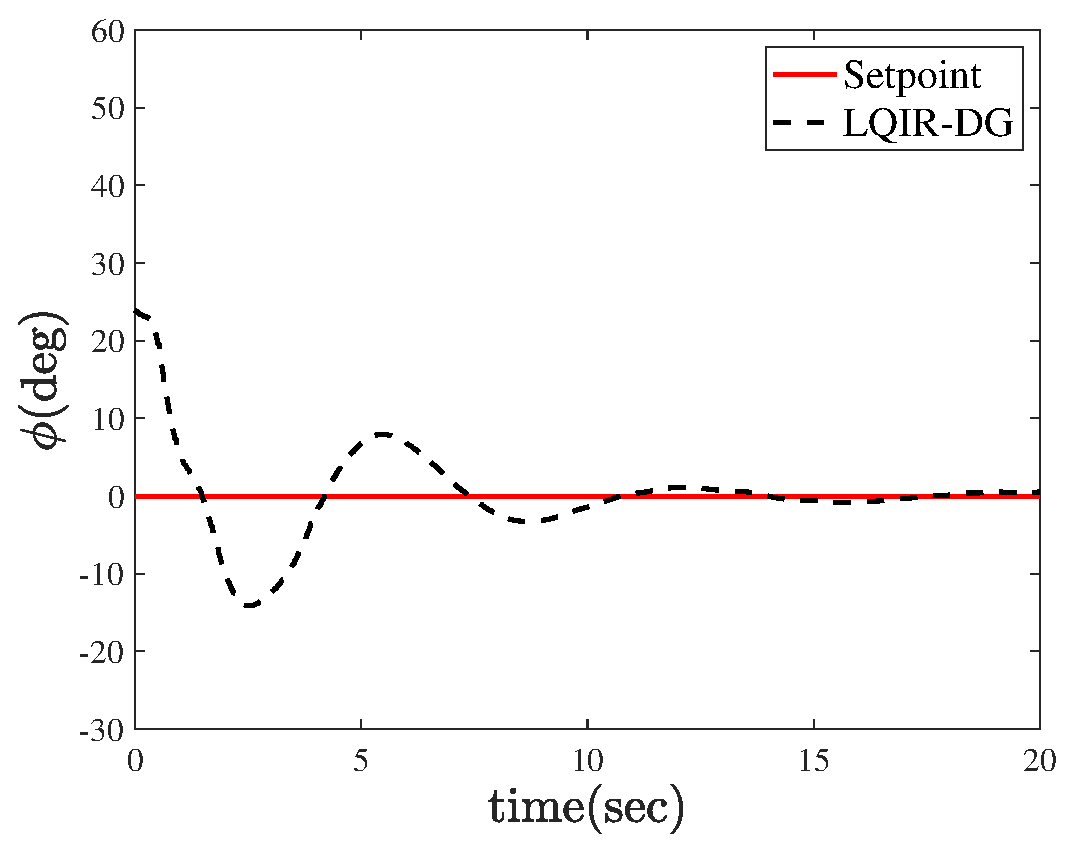
\includegraphics[width=.33\linewidth]{../Figure/implementation/lqidg_roll}}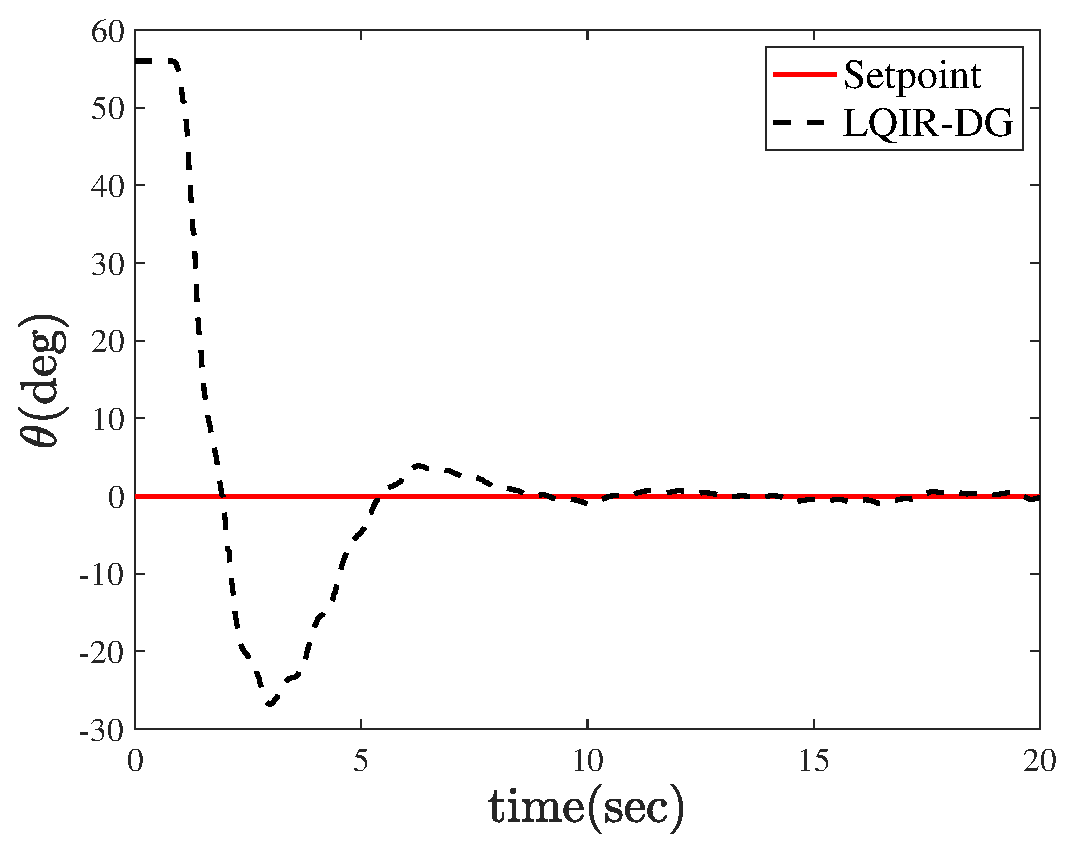
\includegraphics[width=.33\linewidth]{../Figure/implementation/lqidg_pitch}
	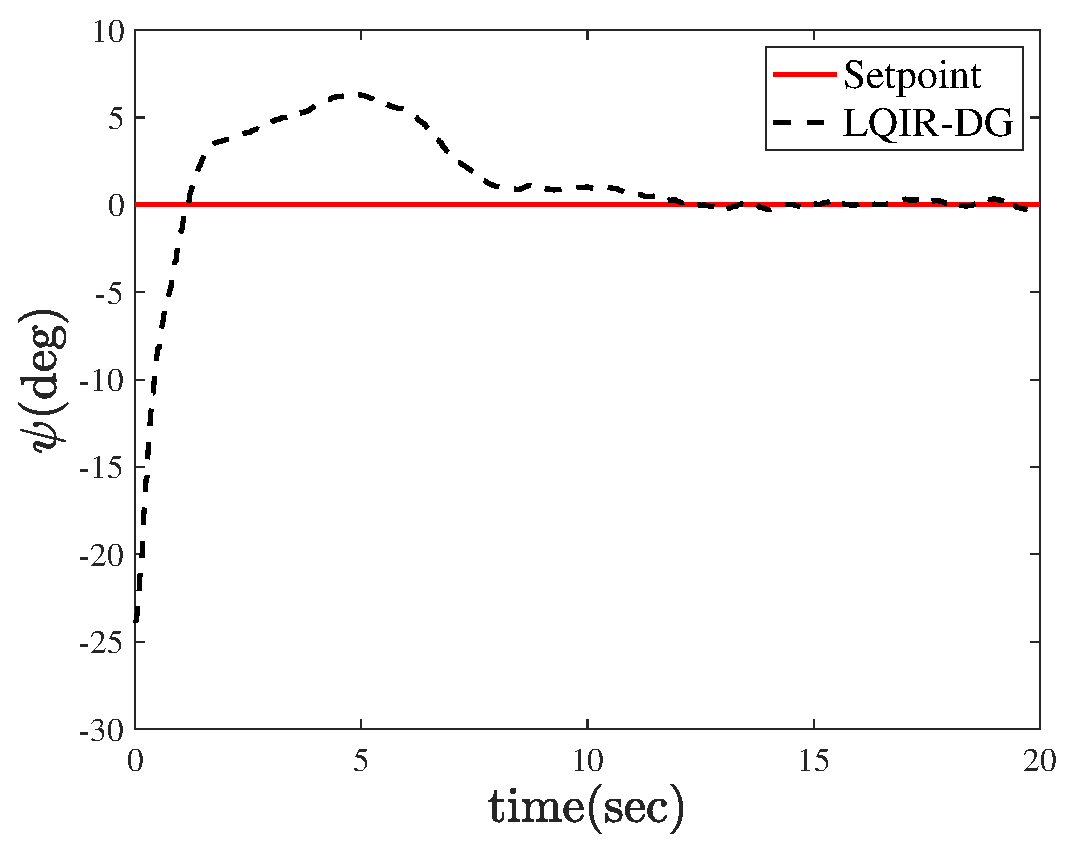
\includegraphics[width=.33\linewidth]{../Figure/implementation/lqidg_yaw}}
	\hfill
	\subfloat[\label{fig:square}]{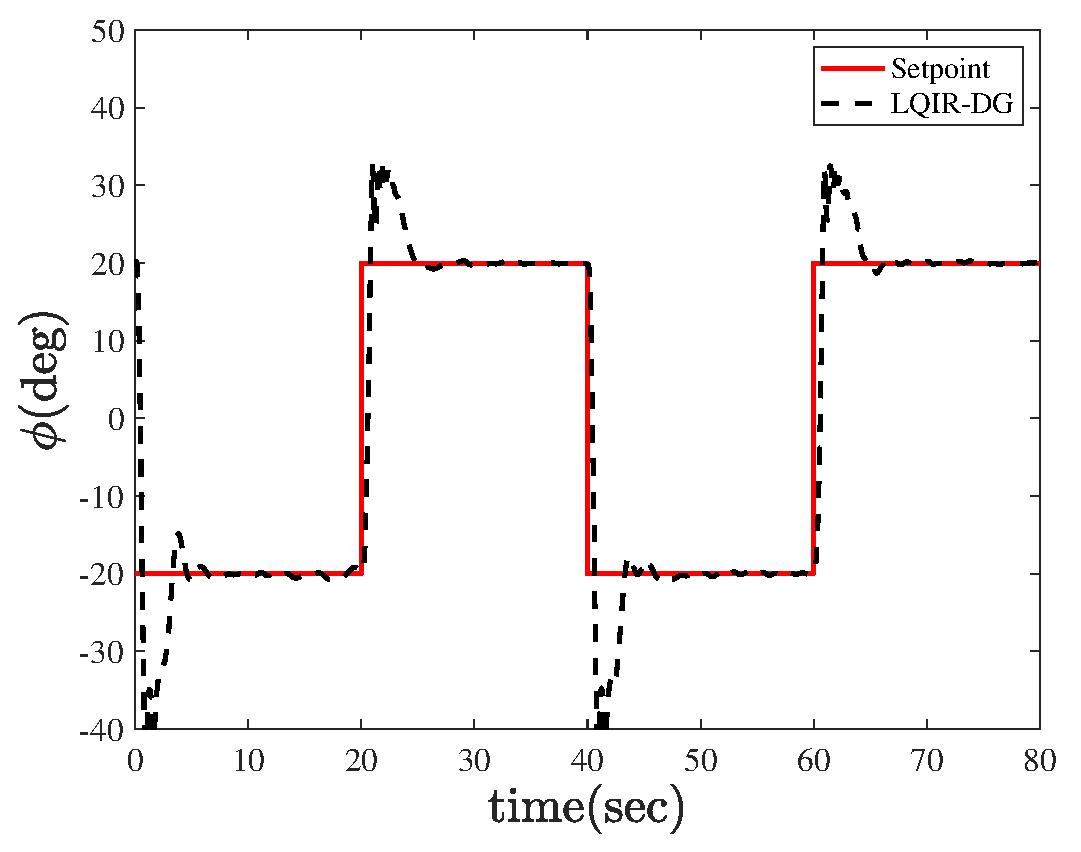
\includegraphics[width=.35\linewidth]{../Figure/implementation/square/lqidg_roll_20}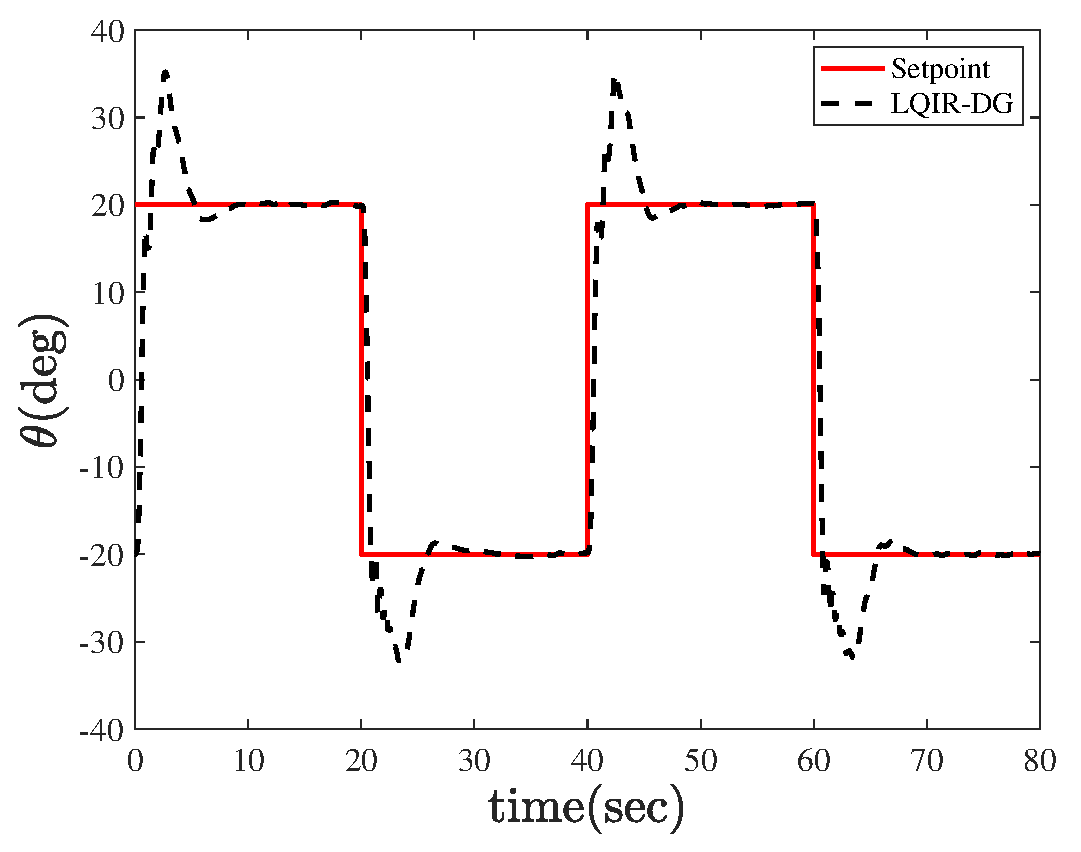
\includegraphics[width=.35\linewidth]{../Figure/implementation/square/lqidg_pitch_20}}
	\caption{Comparison of actual roll and pitch angles with the desired values in \ref{sub@fig:regulation} Regulation \ref{sub@fig:square} Tracking problem.}
	\label{fig:result}
\end{figure}

\begin{figure}[H]
	\vspace{0.3cm}
	\centering
	\subfloat[\label{fig:omega_regulation}]{\includegraphics[width=.25\linewidth]{../Figure/implementation/lqidg_Omega_1}\includegraphics[width=.25\linewidth]{../Figure/implementation/lqidg_Omega_2}\includegraphics[width=.25\linewidth]{../Figure/implementation/lqidg_Omega_3}\includegraphics[width=.25\linewidth]{../Figure/implementation/lqidg_Omega_4}
	}
	\hfil
	\subfloat[\label{fig:omega_square}]{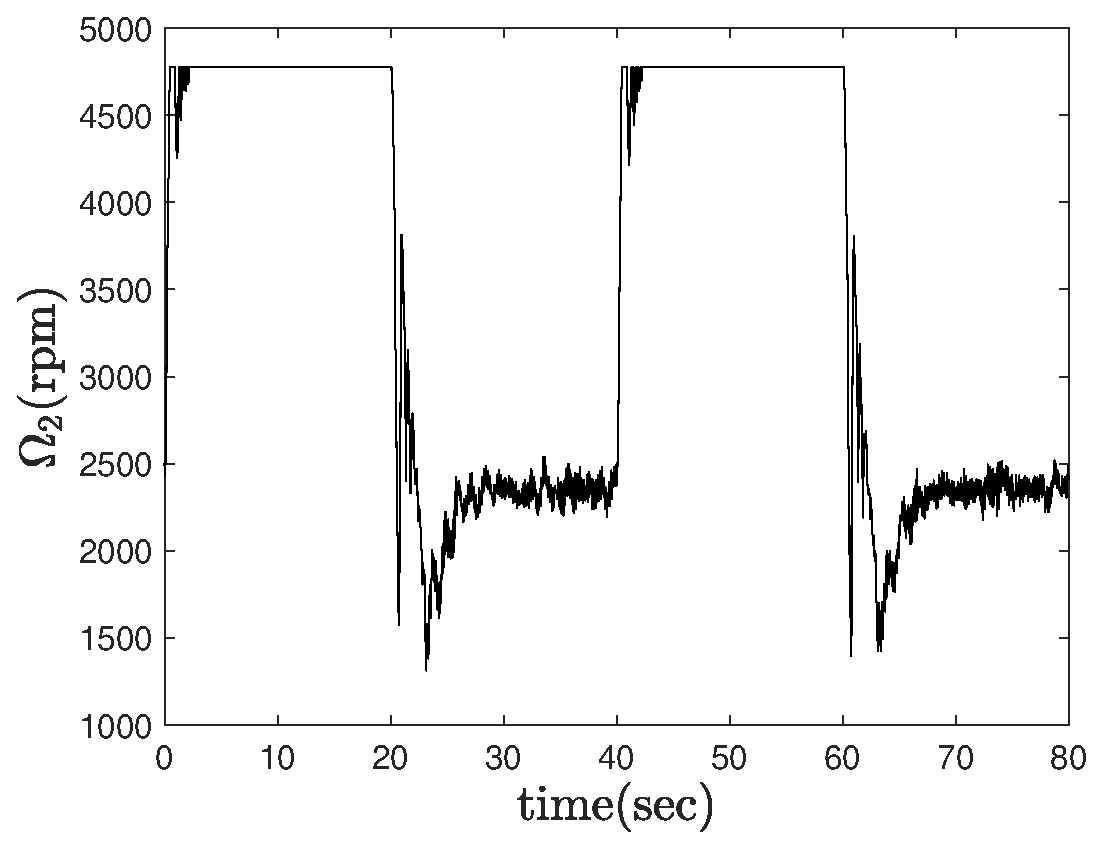
\includegraphics[width=.25\linewidth]{../Figure/implementation/square/lqidg_squre_omega_2}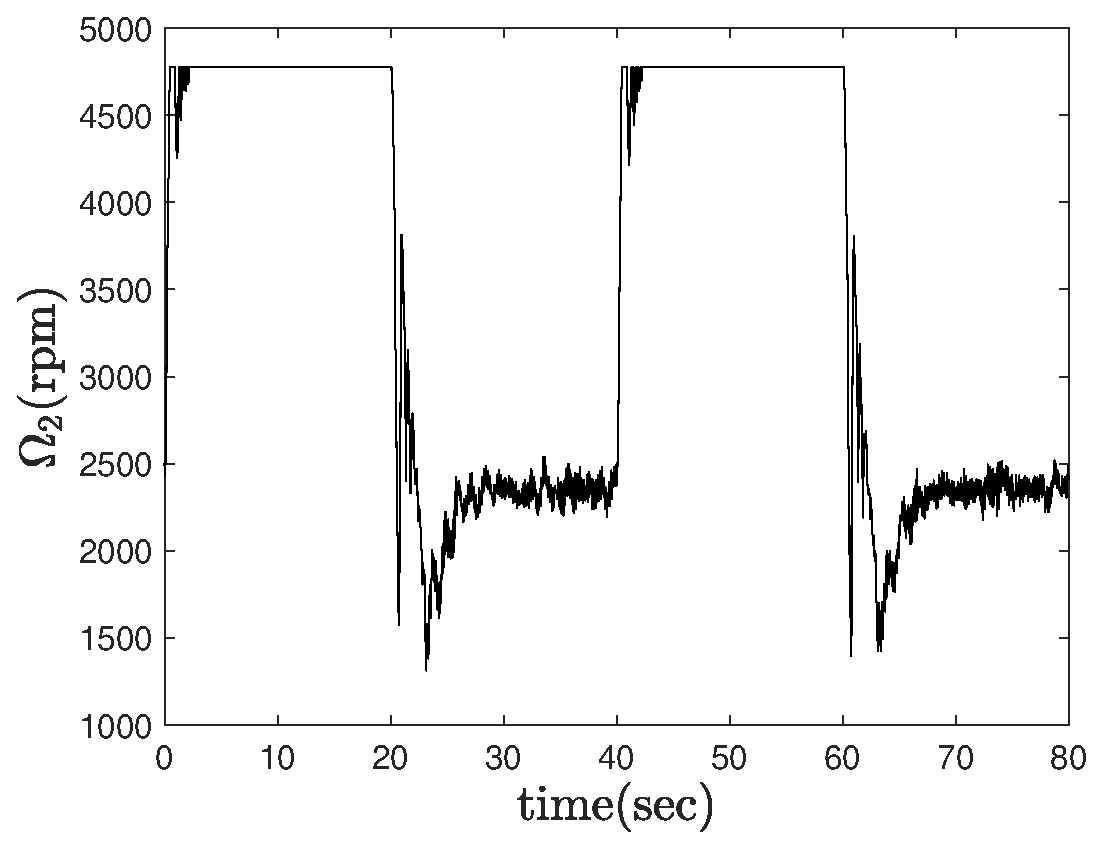
\includegraphics[width=.25\linewidth]{../Figure/implementation/square/lqidg_squre_omega_2}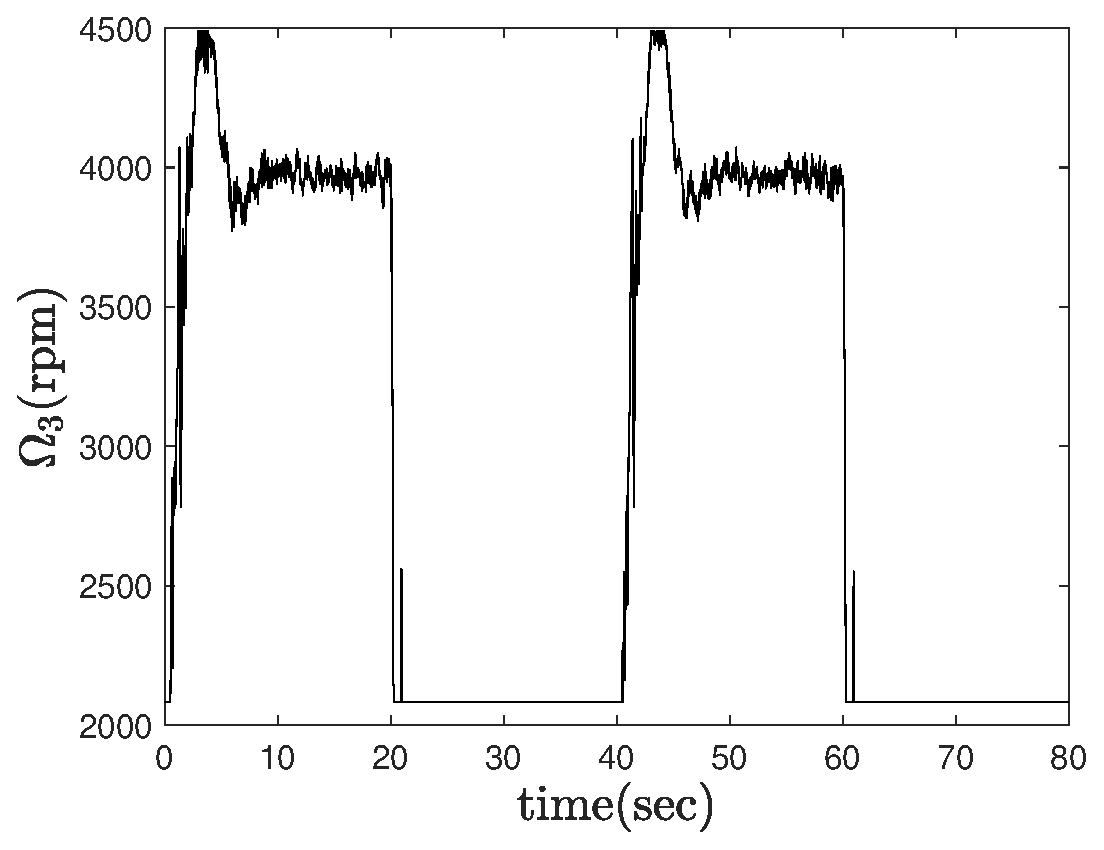
\includegraphics[width=.25\linewidth]{../Figure/implementation/square/lqidg_squre_omega_3}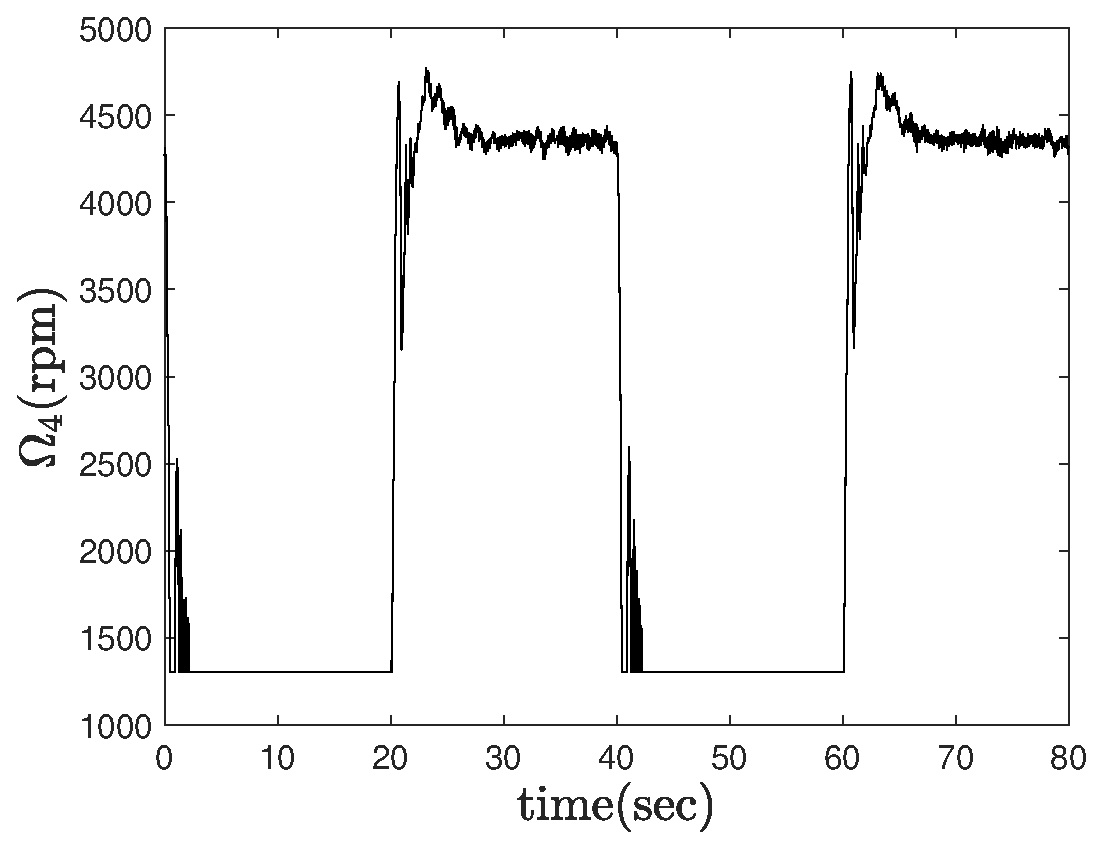
\includegraphics[width=.25\linewidth]{../Figure/implementation/square/lqidg_squre_omega_4}} %%%? didnt describe a and b
	\caption{Rotational velocity  commands in \ref{sub@fig:omega_regulation} Regulation \ref{sub@fig:omega_square} Tracking problems.}
	\label{fig:omega}
\end{figure}
\subsubsection{Investigating the Disturbance Rejection}\label{sec:disturbance}
\noindent Here, the effect of the input disturbance is investigated on the performance of the proposed controller.
The input disturbance, $\mathrm{d_{\Omega_i}}$, is considered as a change in the command of the rotational velocity, modeled as %%%? with or in for input disturbace
\begin{equation}
	\mathrm{d_{\Omega_1}} = \mathrm{d_{\Omega_2}} = -\mathrm{d_{\Omega_3}} = -\mathrm{d_{\Omega_4}} = \begin{cases}
		500~{\mathrm{rpm}} \quad &20<t<60\\
		0 \quad &\mathrm{other}
	\end{cases}
\end{equation}
Figure \ref{fig:disturbance} illustrates the roll and pitch angles in the regulation problem, when the input disturbance occurs. These results indicate that the proposed controller can stabilize the quadrotor platform in the presence of input disturbance.



\begin{figure}[H]
	\centering
	\subfloat{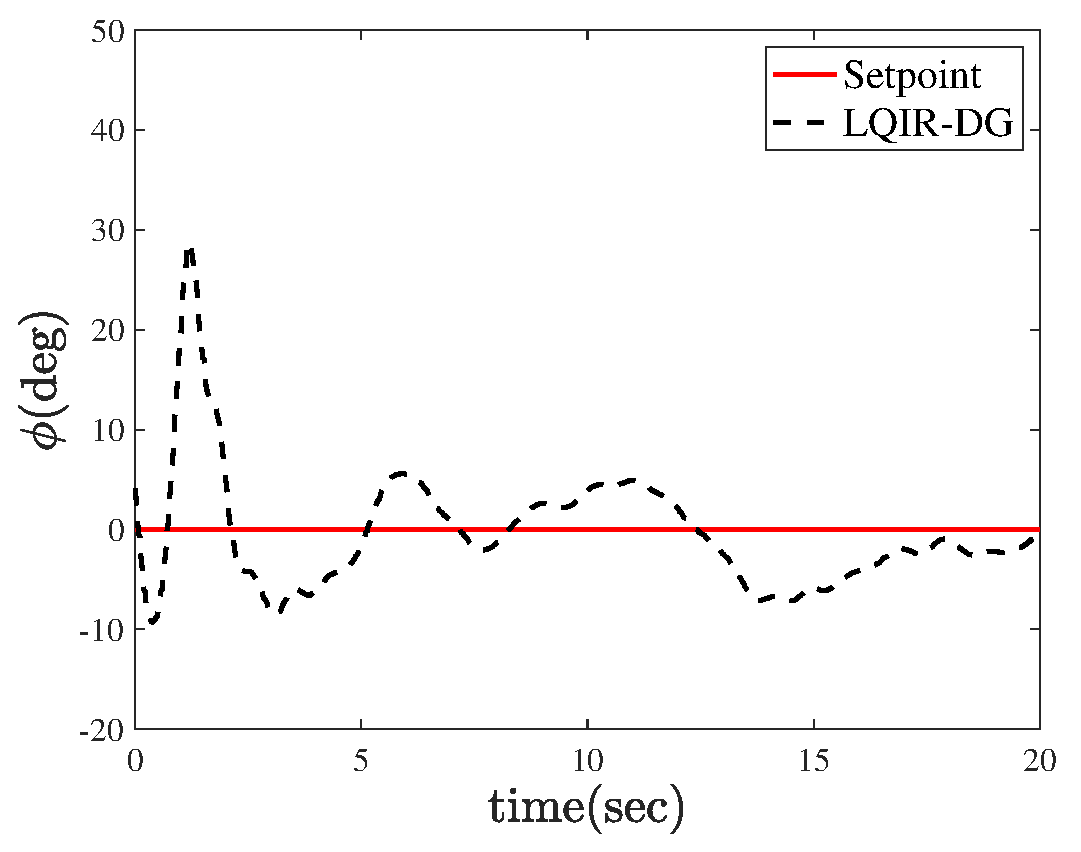
\includegraphics[width=.49\linewidth]{../Figure/implementation/disturbance/lqidg_roll}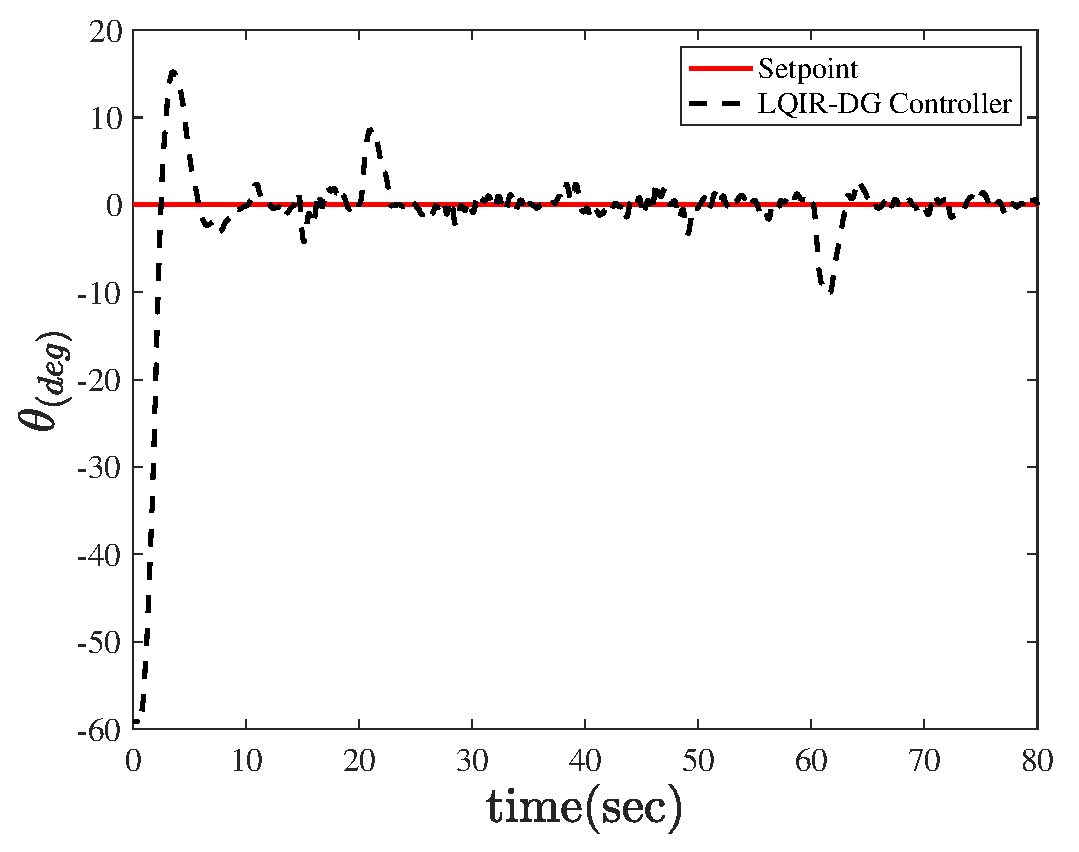
\includegraphics[width=.49\linewidth]{../Figure/implementation/disturbance/lqidg_pitch}
	}
	% \hfill
	% \subfloat[\label{fig:omega_disturbance}]{\includegraphics[width=.23\linewidth]{../Figure/implementation/disturbance/lqidg_Omega_1}\includegraphics[width=.23\linewidth]{../Figure/implementation/disturbance/lqidg_Omega_2}\includegraphics[width=.23\linewidth]{../Figure/implementation/disturbance/lqidg_Omega_3}\includegraphics[width=.23\linewidth]{../Figure/implementation/disturbance/lqidg_Omega_4}}
	
	\caption{Comparison of actual roll and pitch angles with the desired, when the input disturbance occurs.}
	\label{fig:disturbance}
\end{figure}
\subsubsection{Investigating the Impact of Modeling Uncertainty}\label{sec:model-uncertainty}
\noindent The effect of the modeling uncertainty is investigated on the performance of the proposed controller.
To achieve this, 50 and 100 grams weights are added to the roll and pitch axes, respectively, as shown in Figure \ref{fig:quadrotor_with_weight}.
Figure \ref{fig:weight} \ref{sub@fig:weight_roll} compares the desired and the actual roll angle and Figure \ref{fig:weight} \ref{sub@fig:weight_pitch} shows the desired and the actual pitch angle, when the uncertainty of moments of inertia is present.
Moreover, Figure \ref{fig:weight} \ref{sub@fig:omega_weight} shows the rotational velocity commands of the experimental platform, when the model uncertainty is applied.
The implementation results show that the platform outputs converge to the desired values in the presence of the modeling uncertainty.
\begin{figure}[H]
	\centering
	\includegraphics[width=0.45\textwidth]{../Figure/implementation/weight/Quad_with_weight.jpg}
	\caption{Quadrotor 3-DoF platform with added weights.} %%%? is it okey
	\label{fig:quadrotor_with_weight}
%  \end{figure}
%  \begin{figure}[H]
	\centering
	\subfloat[\label{fig:weight_roll}]{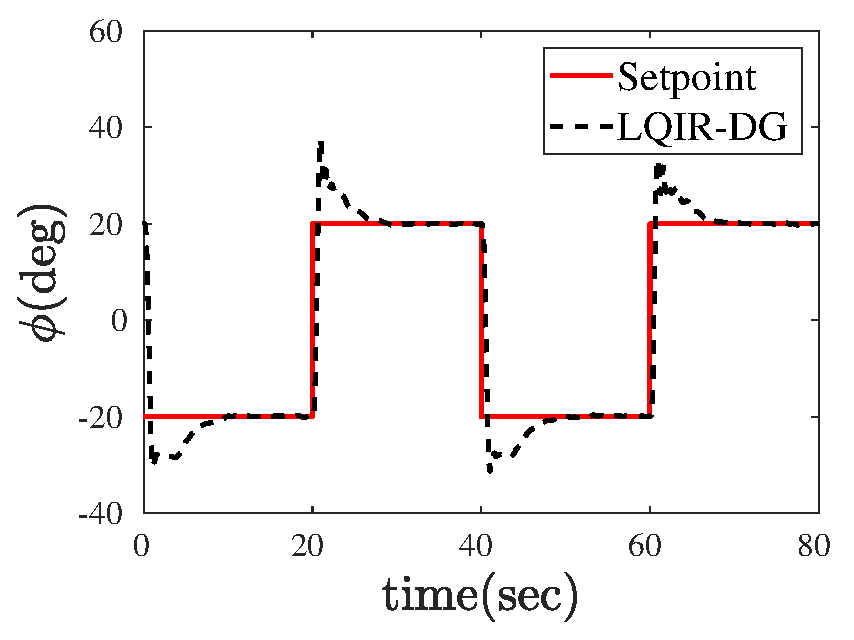
\includegraphics[width=.45\linewidth]{../Figure/implementation/weight/lqidg_roll_20}}\subfloat[\label{fig:weight_pitch}]{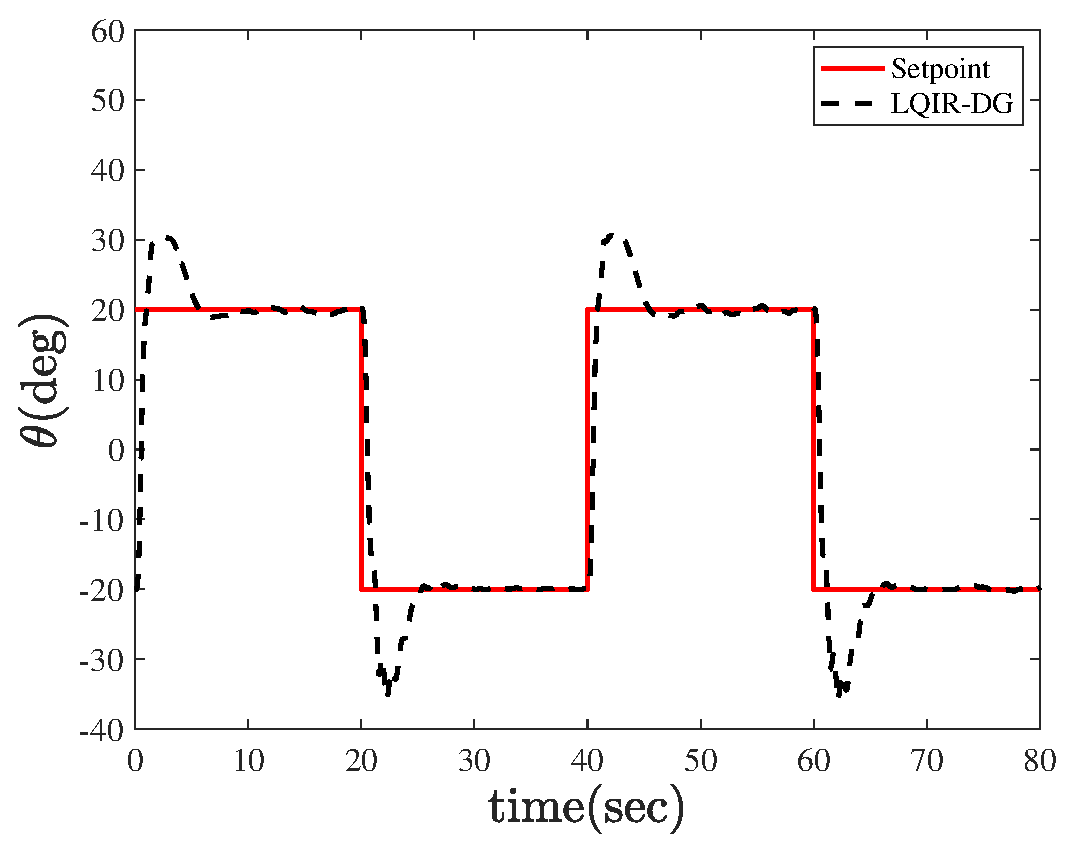
\includegraphics[width=.45\linewidth]{../Figure/implementation/weight/lqidg_pitch_20}
	}
	\hfill
	\subfloat[\label{fig:omega_weight}]{\includegraphics[width=.25\linewidth]{../Figure/implementation/weight/lqidg_Omega_1}\includegraphics[width=.25\linewidth]{../Figure/implementation/weight/lqidg_Omega_2}\includegraphics[width=.25\linewidth]{../Figure/implementation/weight/lqidg_Omega_3}\includegraphics[width=.25\linewidth]{../Figure/implementation/weight/lqidg_Omega_4}}
	\caption{Comparison of actual roll and pitch angles with desired values, when the modeling uncertainty is present.}
	\label{fig:weight}
\end{figure}
\subsubsection{Comparison with the Control Strategies}
\noindent Figure \ref{fig:compare} compares the LQIR-DG controller performance with the PID controller and variant of the LQR strategies such as the LQR and LQIR. 
Moreover, the box plot of all controllers is plotted in Figure \ref{fig:compare_boxplot} for the cost function, introduced in equation \eqref{eq:min_max_cost_function}. %%%? two controller side by side
The median of Root Mean Square Error (RMSE) is shown in the crossline in the box plot.
These results indicate that the proposed controller is able to provide rapid convergence and excellent transient response relative to other controllers for attitude control of the experimental platform.

\begin{figure}[H]
	\centering
	\subfloat[\label{fig:all_roll}]{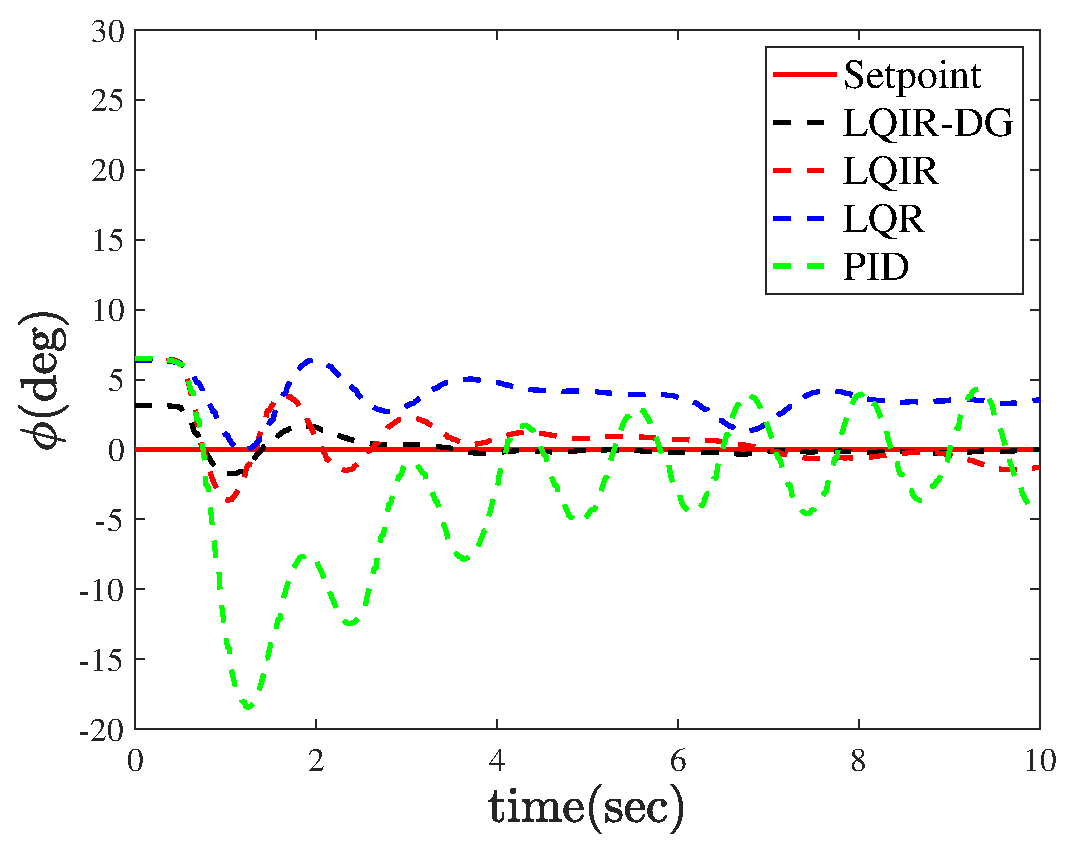
\includegraphics[width=.49\linewidth]{../Figure/implementation/lqidgvslqr/roll}}\subfloat[\label{fig:all_pitch}]{\includegraphics[width=.49\linewidth]{../Figure/implementation/lqidgvslqr/pitch}
	}
	\caption{Comparison of LQIR-DG structure with the variant of LQR and PID in regulation problem: \ref{sub@fig:all_roll} Roll Angle \ref{sub@fig:all_pitch} Pitch Angle.}
	\label{fig:compare}
\end{figure}

\begin{figure}[H]
	\centering
	{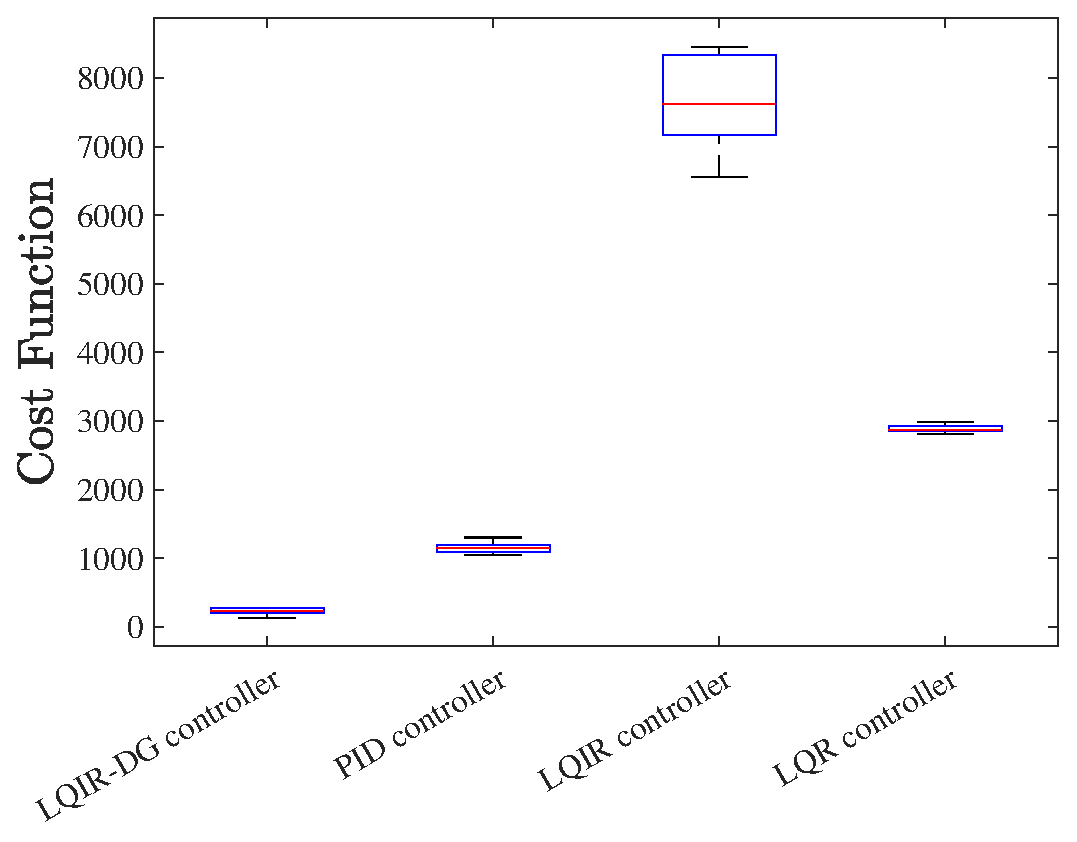
\includegraphics[width=.55\linewidth]{../Figure/implementation/box_plot/lqidgvsboxplot}
	}
	\caption{Box plot of LQIR-DG, LQR, LQIR, and PID controllers.}
	\label{fig:compare_boxplot}
\end{figure}
\section{Conclusion}\label{sec:conclusion}
\noindent In this paper, the linear quadratic integral differential game approach, was used in real-time for attitude control of the platform quadrotor. %%%? for quadrotor
For the implementation of the controller structure, an accurate dynamic model was considered for the experimental platform.
Then, the model parameters were identified using the NSL method.
For evaluation of the proposed method, the regulation and tracking  proposed were successfully performed.
Moreover, the ability of the proposed method was investigated in the rejection of the input disturbance and modeling error in the experimental platform.
Finally, a comparison
was also performed between the results of classical PID, LQR, and LQIR with the proposed method.The implementation results illustrated the excellent performance of the LQIR controller based on the game theory approach in attitude control for the quadrotor platform.
%% The Appendices part is started with the command \appendix;
%% appendix sections are then done as normal sections
%% \appendix

%% \section{}
%% \label{}

%% If you have bibdatabase file and want bibtex to generate the
%% bibitems, please use
%%
 \bibliographystyle{elsarticle-harv} 
 \bibliography{refs}

%% else use the following coding to input the bibitems directly in the
%% TeX file.

% \begin{thebibliography}{00}

%% \bibitem[Author(year)]{label}
%% Text of bibliographic item

% \bibitem[ ()]{}

% \end{thebibliography}
\end{document}

\endinput
%%
%% End of file `elsarticle-template-harv.tex'.
